\documentclass[aspectratio=169]{beamer}

\usepackage{beamerthemesplit}
\usepackage{amsmath}
\usepackage{amsfonts}
\usepackage{amssymb}
\usepackage{cancel}
\usepackage{bussproofs}
\usepackage{graphicx}

% For ⩘ and ⩗ (requires the LuaLaTeX engine)
\usepackage{unicode-math}
\setmathfont{Stix Two Math}

% For highlighting MeTTa code
\usepackage{listings}
\usepackage{color}
\definecolor{mygreen}{rgb}{0,0.6,0}
\definecolor{mymauve}{rgb}{0.58,0,0.82}
\definecolor{dgreen}{rgb}{0,0.5,0}
\definecolor{dblue}{rgb}{0,0,0.5}
\definecolor{dred}{rgb}{0.5,0,0}
\lstset{ %
  backgroundcolor=\color{white},   % choose the background color
  basicstyle=\tiny,                % size of fonts used for the code
  breaklines=true,                 % automatic line breaking only at whitespace
  captionpos=b,                    % sets the caption-position to bottom
  commentstyle=\color{mygreen},    % comment style
  escapeinside={\%*}{*)},          % if you want to add LaTeX within your code
  keywordstyle=\color{blue},       % keyword style
  stringstyle=\color{mymauve},     % string literal style
}

\makeatletter
\newcommand{\tinier}{\@setfontsize{\srcsize}{3.5pt}{3.5pt}}
\makeatother

\makeatletter
\newcommand{\tiniest}{\@setfontsize{\srcsize}{2pt}{2pt}}
\makeatother

\mode<presentation>
{
  \usetheme{AnnArbor}
  \usecolortheme{crane}
}

\usepackage[english]{babel}
%% \usepackage[latin1]{inputenc}
\usepackage{times}
\usepackage[T1]{fontenc}

\title{Meta-Reasoning in MeTTa\\
  {\tiny for Inference Control via Provably Pruning the Search Tree}}

\author{Nil Geisweiller}

\institute[SingularityNET OpenCog Foundations]
{
  \begin{center}
    %% 
\includegraphics[scale=0.1]{pics/trueagi-logo-small.png}\\
    
\includegraphics[scale=0.2]{pics/snet-logo.png}\\[1cm]
    Artificial Intelligence and Theorem Proving 2024 (AITP-24)
  \end{center}
}

\date[AITP-24]

\begin{document}

\lstset{language=Lisp}

\begin{frame}
  \maketitle
\end{frame}

\section{Introduction}

\subsection{SingularityNET: AI service composition}

\begin{frame}[fragile]
  %% <BEGIN-SPEECH> Let me briefly introduce myself, I'm Nil Geisweiller,
  %% I work at the SingularityNET Foundation, I do a lot of AI, though
  %% I'm mostly interested in reasoning.  So more specifically why do I
  %% care about automated theorem proving, there are several reasons, but
  %% an important one is because at the SingularityNET Foundation we
  %% offer a market place of AI services and the ability to automatically
  %% connect AI services together, and so if you view AI services as
  %% functions, and their types as specifications, then synthesizing
  %% compositions of AI services is identical to doing theorem
  %% proving. <END-SPEECH>

  \begin{columns}
    \begin{column}{7cm}

      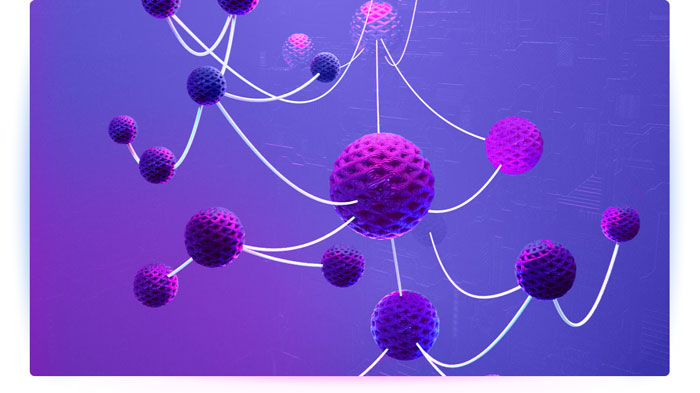
\includegraphics[scale=0.3]{pics/AI-Domain-Specific-Language-DSL-Image.jpg}

    \end{column}

    \vrule

    \begin{column}{7cm}

      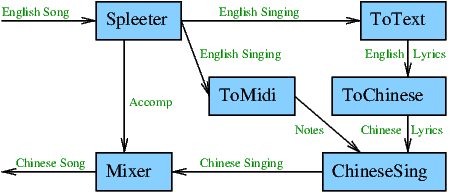
\includegraphics[scale=0.4]{pics/EnglishToChineseSong.png}

      \begin{lstlisting}
 -------------------------------------------------
 (-> (: $s (SongIn "English")) (SongIn "Chinese"))
      \end{lstlisting}

    \end{column}

  \end{columns}
\end{frame}

\subsection{Outline}

\begin{frame}

  %% <BEGIN-SPEECH> My presentation is more motivational than anything
  %% else.  What I am going to present is very early stage, I
  %% don't have great results to show you, but I'd like to sell you
  %% two things:

  %% 1. MeTTa, a programming language that we're developing at
  %% SingularityNET.

  %% 2. The old idea of meta-reasoning.

  %% Personally the first time I encountered that idea of
  %% meta-reasoning was in the Goedel machine paper of Juergen
  %% Schimdhubber.  I'm not saying it is the first time it appeared on
  %% this world, but it was the first time I encountered it.

  \begin{itemize}
  \item MeTTa
  \item Meta-reasoning
  \end{itemize}
\end{frame}

\subsection{G\"odel Machine}

\begin{frame}[fragile]
  %% <BEGIN-SPEECH> I'm going to recall briefly what is a Goedel
  %% machine.  Very early on, Juergen was obsessed with the problem of
  %% intelligence bootstrapping.  The problem goes as follows, let's
  %% say I have a machine that is trying to learn how to drive a car,
  %% but learning is difficult, you've got hyper parameters to tune so
  %% that it can do that efficiently, and doing that manually is time
  %% consuming and difficult too.  So, OK no problem, you add a second
  %% machine to learn how to tune those hyper parameters, but that
  %% machine also has hyper parameters, that if you could tune just
  %% right you'd be able to make learn that efficiently, OK so you add
  %% a third machine, and yeah it potentially never ends.  So after
  %% years of thinking hard and deep about this problem, Juergen found
  %% a solution, which is essentially the combination of 3 ideas:

  %% 1. Let's merge all these machines into one.

  %% 2. Let's have the action set not just about the external world, such
  %% as driving a car, but also about the internal world, specifically
  %% actions to rewrite the content of any memory cell of the machine.

  %% 3. And the third and crucial idea is: only allow actions to get
  %% triggered if we have a mathematical proof that it is indeed a good
  %% idea.

  %% And so that last idea is what I'm trying to realize in the
  %% context of guiding automated theorem proving, specifically given
  %% a theorem prover facing all different paths that can be explored
  %% to find a proof, my system only allows to pursue the paths that
  %% have been mathematically proven to be worth pursuing.  So the
  %% pruner is itself a theorem prover.

  %% <END-SPEECH>

  \begin{columns}[T]
    \begin{column}{2cm}%\column{5cm}
    \only<1>{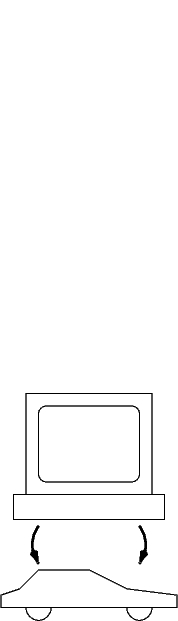
\includegraphics[scale=0.3]{pics/computer-driving.png}}
    \only<2>{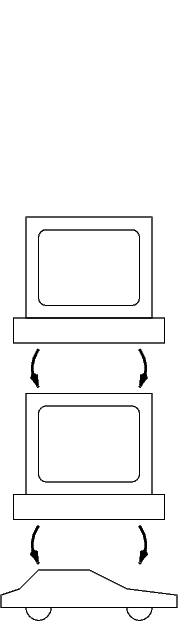
\includegraphics[scale=0.3]{pics/meta-computer-driving.png}}
    \only<3>{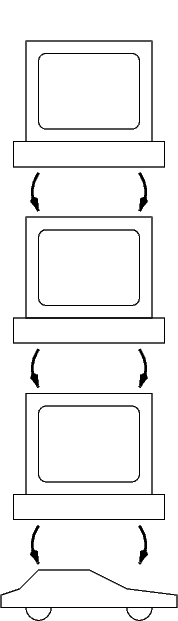
\includegraphics[scale=0.3]{pics/meta-meta-computer-driving.png}}
    \only<4->{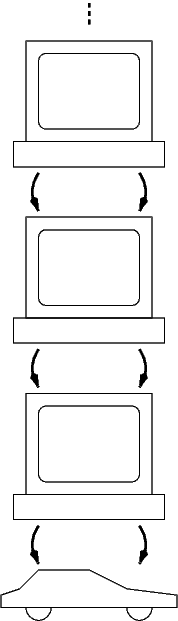
\includegraphics[scale=0.3]{pics/inf-computer-driving.png}}
    \end{column}

    \vrule{}

    \begin{column}{8cm}
      \visible<5->{G\"odel Machine \emph{(J\"urgen Schmidhuber, 2003)}}
      \begin{itemize}
      \item<6-> Merge all machines into one.
      \item<7-> Internal actions to action space.
      \item<8-> Mathematical proof $\Rightarrow$ trigger action.
      \end{itemize}
      \begin{center}
        \only<6>{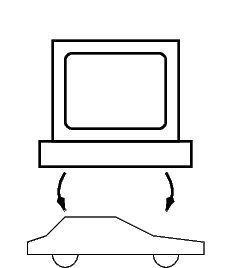
\includegraphics[scale=0.3]{pics/goedel-machine1.png}}
        \only<7>{
\includegraphics[scale=0.3]{pics/goedel-machine2.png}}
        \only<8>{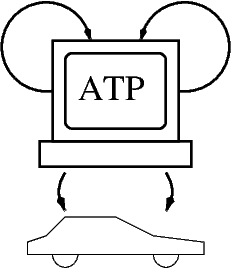
\includegraphics[scale=0.3]{pics/goedel-machine3.png}}
      \end{center}
    \end{column}
  \end{columns}

\end{frame}

\section{Meta-reasoning}

\subsection{Backward chaining}

\begin{frame}

  %% <BEGIN-SPEECH> So you all know how a backward chainer works.  You
  %% start from a theorem, and you expand your proof backward till you
  %% reach the axioms.

  %% Of course, it's not that simple because at each expansion step
  %% you usually have multiple rules to choose from and therefore many
  %% paths to explore, and most of them will fail.  So you have to
  %% intelligently prune the search.  And I don't know for you, but
  %% for me, I cannot think of anything more intelligent than a
  %% reasoning system, at least in potential.  So let's do that, let's
  %% use a reasoning system as a control mechanism! <END-SPEECH>

  \begin{columns}

    \column{1cm}

    {\tiny
    \begin{prooftree}
      \AxiomC{$\text{Theorem}$}
    \end{prooftree}
    }

    \column{1cm}

    \pause

    \begin{center}
      \visible<4>{$\nearrow$}\\
      $\rightarrow$\\
      \visible<4>{$\searrow$}\\
    \end{center}

    \column{4cm}

    \begin{center}
      \visible<4>{$\ldots$}
    \end{center}

    {\tiny
    \begin{prooftree}
      \AxiomC{$\text{Lemma}_j$}
      \AxiomC{$\text{Lemma}_k$}
      \RightLabel{($R_i$)}
      \BinaryInfC{$\text{Theorem}$}
    \end{prooftree}
    }

    \begin{center}
      \visible<4>{$\ldots$}
    \end{center}

    \column{1cm}

    \pause

    \begin{center}
      \visible<4>{$\nearrow$}\\
      $\rightarrow$\\
      \visible<4>{$\searrow$}\\
    \end{center}

    \column{8cm}

    \begin{center}
      \visible<4>{$\ldots$}\\
      \visible<4>{$\ldots$}\\
      \visible<4>{$\ldots$}
    \end{center}

    {\tiny
      \begin{prooftree}
        \AxiomC{}
        %% \RightLabel{($A_l$)}
        \UnaryInfC{$\text{Axiom}_l$}
        \AxiomC{}
        %% \RightLabel{($A_m$)}
        \UnaryInfC{$\text{Axiom}_m$}
        \RightLabel{($R_n$)}
        \BinaryInfC{$\text{Lemma}_j$}
        \AxiomC{}
        %% \RightLabel{($A_i$)}
        \UnaryInfC{$\text{Axiom}_n$}
        \AxiomC{}
        %% \RightLabel{($A_j$)}
        \UnaryInfC{$\text{Axiom}_o$}
        \RightLabel{($R_k$)}
        \BinaryInfC{$\text{Lemma}_k$}
        \RightLabel{($R_i$)}
        \BinaryInfC{$\text{Theorem}$}
      \end{prooftree}
    }

    \begin{center}
      \visible<4>{$\ldots$}\\
      \visible<4>{$\ldots$}\\
      \visible<4>{$\ldots$}
    \end{center}

  \end{columns}

\end{frame}

\subsection{Backward Chaining with control}

\begin{frame}

  %% <BEGIN-SPEECH> NEXT <END-SPEECH>

  \begin{columns}

    \column{1cm}

    {\small
    \begin{prooftree}
      \AxiomC{$\text{Theorem}$}
    \end{prooftree}
    }

    \column{3cm}

    \begin{center}
      $\nearrow R_1$\\[0.5cm]
      $\searrow R_2$
    \end{center}

    \column{1cm}

    \column{5cm}

    {\small
    \begin{prooftree}
      \AxiomC{$\text{Lemma}_j$}
      \AxiomC{$\text{Lemma}_k$}
      \RightLabel{($R_1$)}
      \BinaryInfC{$\text{Theorem}$}
    \end{prooftree}
    }

    \vphantom{}\\[1cm]

    {\small
    \begin{prooftree}
      \AxiomC{$\text{Lemma}_l$}
      \AxiomC{$\text{Lemma}_m$}
      \RightLabel{($R_2$)}
      \BinaryInfC{$\text{Theorem}$}
    \end{prooftree}
    }

    \column{1cm}

    \column{1cm}

  \end{columns}
\end{frame}

\begin{frame}

  %% <BEGIN-SPEECH> NEXT <END-SPEECH>

  \begin{columns}

    \column{1cm}

    {\small
    \begin{prooftree}
      \AxiomC{$\text{Theorem}$}
    \end{prooftree}
    }

    \column{3cm}

    {\tiny
      \begin{prooftree}
        \AxiomC{}
        \UnaryInfC{$\vdots$}
        \AxiomC{}
        \UnaryInfC{$\vdots$}
        \AxiomC{}
        \UnaryInfC{$\vdots$}
        \TrinaryInfC{$(\text{Continue}\ \text{Context}\ R_1)$}
    \end{prooftree}}

    \begin{center}
      $\nearrow R_1$\\[0.5cm]
      $\searrow R_2$
    \end{center}

    {\tiny
      \begin{prooftree}
        \AxiomC{$?$}
        \AxiomC{$?$}
        \AxiomC{$?$}
        \TrinaryInfC{$(\text{Continue}\ \text{Context}\ R_2)$}
    \end{prooftree}}

    \column{1cm}

    \begin{center}
      \color{dgreen}{$\rightarrow$}\\[2cm]
      \color{dred}{$\not{\rightarrow}$}
    \end{center}

    \column{5cm}

    \color{dgreen}{
    {\small
    \begin{prooftree}
      \AxiomC{$\text{Lemma}_j$}
      \AxiomC{$\text{Lemma}_k$}
      \RightLabel{($R_1$)}
      \BinaryInfC{$\text{Theorem}$}
    \end{prooftree}
    }}

    \vphantom{}\\[1cm]

    \color{dred}{
    {\small
    \begin{prooftree}
      \AxiomC{$\text{Lemma}_l$}
      \AxiomC{$\text{Lemma}_m$}
      \RightLabel{($R_2$)}
      \BinaryInfC{$\text{Theorem}$}
    \end{prooftree}
    }}

    \pause

    \column{1cm}
    \begin{center}
      $\nearrow$\\
      $\rightarrow$\\
      $\searrow$\\[2cm]
    \end{center}
    \vphantom{}

    \column{1cm}
    \begin{center}
      $\dots$\\
      $\dots$\\
      $\dots$\\[2cm]
    \end{center}
    \vphantom{}

  \end{columns}
\end{frame}

\section{MeTTa: Meta Type Talk}

\subsection{Functional Logic Programming}

\begin{frame}[fragile]
  %% <BEGIN-SPEECH> In order to show you that in more detail I need to
  %% explain to you what is MeTTa, the programming language I've used to
  %% carry out these experiments. <END-SPEECH>

  \frametitle{MeTTa: Meta Type Talk}

  \begin{columns}

    \column{7cm}
    \begin{itemize}
    \item Functional and logic programming
    \item Non-determinism (like Curry)
    \item Unification (like Prolog)
    \item Gradual typing
    \item Self-modifiable
    \item Concurrency
    \item Scalable
    \end{itemize}

    \column{7cm}

    \begin{lstlisting}
      ;; Bit strings
      (= (bits Z) Nil)
      (= (bits (S $k)) (Cons 0 (bits $k)))
      (= (bits (S $k)) (Cons 1 (bits $k)))

      ;; Generate all 3-bit strings
      !(bits (S (S (S Z))))
    \end{lstlisting}

    \begin{center}
      $\Downarrow$
    \end{center}

    \begin{lstlisting}
      [(Cons 0 (Cons 0 (Cons 0 Nil)))
       (Cons 0 (Cons 0 (Cons 1 Nil)))
       (Cons 0 (Cons 1 (Cons 0 Nil)))
       (Cons 0 (Cons 1 (Cons 1 Nil)))
       (Cons 1 (Cons 0 (Cons 0 Nil)))
       (Cons 1 (Cons 0 (Cons 1 Nil)))
       (Cons 1 (Cons 1 (Cons 0 Nil)))
       (Cons 1 (Cons 1 (Cons 1 Nil)))]
    \end{lstlisting}

  \end{columns}

\end{frame}

%% \begin{frame}[fragile]
%%   %% <BEGIN-SPEECH> In order to show you that in more detail I need to
%%   %% explain to you what is MeTTa, the programming language I've used to
%%   %% carry out these experiments. <END-SPEECH>

%%   \frametitle{MeTTa: Meta Type Talk}

%%   \begin{columns}

%%     \column{7cm}
%%     \begin{itemize}
%%     \item Functional and logic programming
%%     \item Non-determinism (like Curry)
%%     \item Unification (like Prolog)
%%     \item Gradual typing
%%     \item Self-modifiable
%%     \item Concurrency
%%     \item Scalable
%%     \end{itemize}

%%     \column{7cm}

%%     \begin{lstlisting}
%%       ;; Bit strings
%%       (= (bits Z) Nil)
%%       (= (bits (S $k)) (Cons 0 (bits $k)))
%%       (= (bits (S $k)) (Cons 1 (bits $k)))

%%       ;; Generate all 3-bit strings
%%       ;; !(bits (S (S (S Z))))
%%       !(bits ($x ($y ($z Z))))
%%     \end{lstlisting}

%%     \begin{center}
%%       $\Downarrow$
%%     \end{center}

%%     \begin{lstlisting}
%%       [(Cons 0 (Cons 0 (Cons 0 Nil)))
%%        (Cons 0 (Cons 0 (Cons 1 Nil)))
%%        (Cons 0 (Cons 1 (Cons 0 Nil)))
%%        (Cons 0 (Cons 1 (Cons 1 Nil)))
%%        (Cons 1 (Cons 0 (Cons 0 Nil)))
%%        (Cons 1 (Cons 0 (Cons 1 Nil)))
%%        (Cons 1 (Cons 1 (Cons 0 Nil)))
%%        (Cons 1 (Cons 1 (Cons 1 Nil)))]
%%     \end{lstlisting}

%%   \end{columns}

%% \end{frame}

%% \begin{frame}[fragile]
%%   %% <BEGIN-SPEECH> In order to show you that in more detail I need to
%%   %% explain to you what is MeTTa, the programming language I've used to
%%   %% carry out these experiments.
%%   %%
%%   %% So MeTTa stands for Meta Type Talk, it is a functional logic
%%   %% programming language.
%%   %%
%%   %% It supports non-determinism.  Here's an example of a program that
%%   %% generates all 3-bit strings by taking advantage of non-determinism.
%%   %%
%%   %% It supports full syntactic unification, so if you replace the three
%%   %% Ss in the call of bits by variables, it will still output the same
%%   %% thing, because the matching occurs on both sides.
%%   %%
%%   %% It supports gradual typing, so you can add type annotations but you
%%   %% don't have to.  It's not dynamically typed, it is strongly typed,
%%   %% but in some type checking will occur at run-time not just at
%%   %% compile time, because...
%%   %%
%%   %% It is self-modifiable, so if you wish to remove, add or modify
%%   %% functions at run-time, you can do it.
%%   %%
%%   %% And last but not least it will soon have support for concurrency and
%%   %% it should scale incredibly well, Adam Vandervost who's here is doing
%%   %% some very impressive work on that.
%%   %%
%%   %% <END-SPEECH>

%%   \frametitle{MeTTa: Meta Type Talk}

%%   \begin{columns}

%%     \column{7cm}
%%     \begin{itemize}
%%     \item Functional and logic programming
%%     \item Non-determinism (like Curry)
%%     \item Unification (like Prolog)
%%     \item Gradual typing
%%     \item Self-modifiable
%%     \item Concurrency
%%     \item Scalable
%%     \end{itemize}

%%     \column{7cm}

%%     \begin{lstlisting}
%%       ;; Bit strings
%%       (: bits (-> Nat (List Number)))
%%       (= (bits Z) Nil)
%%       (= (bits (S $k)) (Cons 0 (bits $k)))
%%       (= (bits (S $k)) (Cons 1 (bits $k)))

%%       ;; Generate all 3-bit strings
%%       ;; !(bits (S (S (S Z))))
%%       !(bits ($x ($y ($z Z))))
%%     \end{lstlisting}

%%     \begin{center}
%%       $\Downarrow$
%%     \end{center}

%%     \begin{lstlisting}
%%       [(Cons 0 (Cons 0 (Cons 0 Nil)))
%%        (Cons 0 (Cons 0 (Cons 1 Nil)))
%%        (Cons 0 (Cons 1 (Cons 0 Nil)))
%%        (Cons 0 (Cons 1 (Cons 1 Nil)))
%%        (Cons 1 (Cons 0 (Cons 0 Nil)))
%%        (Cons 1 (Cons 0 (Cons 1 Nil)))
%%        (Cons 1 (Cons 1 (Cons 0 Nil)))
%%        (Cons 1 (Cons 1 (Cons 1 Nil)))]
%%     \end{lstlisting}

%%   \end{columns}

%% \end{frame}

\section{MeTTa example}

\subsection{Backward chainer}

%% <BEGIN-SPEECH>
%% Let me show you what we can do with MeTTa, so this is a backward
%% chainer, that all, the reason it is possible to write a backward
%% chainer so compactly comes from

%% 1. non-determinism.  You see the two definitions of bc, the
%% interpreter it not going to take one or the other, it's going to take
%% both.  But where it becomes really powerful is when you combine
%% non-determinism with recursion because it creates the space of paths
%% that the interpreter can take, a bit like a fractal.

%% 2. unification, this let operator doesn't just do assignment, it's
%% actually a full unification.

%% OK, so let's add a theory to that backward chainer, here is a simple
%% one.

%% And, query the backward chainer with a theorem.

%% Alright, so that was a pretty simple example, but we can even go further.
%% <END-SPEECH>

\begin{frame}[fragile]
  \begin{lstlisting}
;; Backward chainer
(= (bc $kb $_ (: $prf $ccln)) (match $kb (: $prf $ccln) (: $prf $ccln)))
(= (bc $kb (S $k) (: ($prfabs $prfarg) $ccln))
   (let* (((: $prfabs (-> $prms $ccln)) (bc $kb $k (: $prfabs (-> $prms $ccln))))
          ((: $prfarg $prms) (bc $kb $k (: $prfarg $prms))))
     (: ($prfabs $prfarg) $ccln)))
  \end{lstlisting}

  \pause

  \begin{lstlisting}
;; Knowledge base
!(bind! &kb (new-space))
!(add-atom &kb (: AK (-> $a (-> $b $a))))
!(add-atom &kb (: AS (-> (-> $a (-> $b $c)) (-> (-> $a $b) (-> $a $c)))))
  \end{lstlisting}

  \pause

  \begin{lstlisting}
;; Query
!(bc &kb (S (S Z)) (: $prf (-> $a $a)))
  \end{lstlisting}

  \pause

  \begin{lstlisting}
;; Results
[(: ((AS AK) AK) (-> $a $a))
 ...]
  \end{lstlisting}

\end{frame}

\subsection{Backward chainer with dependent types and lambda abstraction}

\begin{frame}[fragile]

  %% <BEGIN-SPEECH>
  %% Here is an example of a backward chainer including lambda
  %% abstraction.  I don't have time to explain it, but I just want to
  %% show you want I can do with it.
  %% <END-SPEECH>

  \begin{lstlisting}
;; Backward chainer with dependent types and lambda abstraction

;;;;;;;;;;;;;;;;
;; Base cases ;;
;;;;;;;;;;;;;;;;

;; Match the knowledge base
(= (bc $kb $env $idx $_ (: $prf $thrm))
   (match $kb (: $prf $thrm) (: $prf $thrm)))
;; Match the environment
(= (bc $kb $env $idx $_ (: $prf $thrm))
   (match' $env (: $prf $thrm) (: $prf $thrm)))

;;;;;;;;;;;;;;;;;;;;;
;; Recursive steps ;;
;;;;;;;;;;;;;;;;;;;;;

;; Proof application
(= (bc $kb $env $idx (S $k) (: ($prfabs (: $prfarg $prms)) $thrm))
   (let* (((: $prfabs (-> (: $prfarg $prms) $thrm))
           (bc $kb $env $idx $k (: $prfabs (-> (: $prfarg $prms) $thrm))))
          ((: $prfarg $prms)
           (bc $kb $env $idx $k (: $prfarg $prms))))
     (: ($prfabs (: $prfarg $prms)) $thrm)))
;; Proof abstraction
(= (bc $kb $env $idx (S $k) (: (\ $idx $prfbdy) (-> (: $idx $prms) $thrm)))
   (let (: $prfbdy $thrm)
     (bc $kb (Cons (: $idx $prms) $env) (s $idx) $k (: $prfbdy $thrm))
     (: (λ $idx $prfbdy) (-> (: $idx $prms) $thrm))))
  \end{lstlisting}

\end{frame}

\subsection{Prove properties over programs}

%% <BEGIN-SPEECH> So given a theory about programming, which is partially
%% given here, I can prove properties over programs, such as that
%% doubling any natural number returns a even number.
%% <END-SPEECH>

\begin{frame}[fragile]

  \begin{lstlisting}
;; Equality is transitive
!(add-atom &kb (: Trans (-> (: $prf1 (=== $x $y))     ; Premise 1
                            (-> (: $prf2 (=== $y $z)) ; Premise 2
                                (=== $x $z)))))       ; Conclusion

;; Equality is symmetric
!(add-atom &kb (: Sym (-> (: $prf (=== $x $y)) ; Premise
                          (=== $y $x))))       ; Conclusion

;; Equality respects function application
!(add-atom &kb (: Cong (-> (: $f (-> (: $_ $a) $b))                 ; Premise 1
                           (-> (: $x $a)                            ; Premise 2
                               (-> (: $x' $a)                       ; Premise 3
                                   (-> (: $prf (=== $x $x'))        ; Premise 4
                                       (=== ($f $x) ($f $x')))))))) ; Conclusion

;; Rule of replacement
!(add-atom &kb (: Replace (-> (: $prf1 (=== $x $x')) ; Premise 1
                              (-> (: $prf2 $x)       ; Premise 2
                                  $x'))))            ; Conclusion

;; Define double
!(add-atom &kb (: double (-> (: $k N) N)))
!(add-atom &kb (: double_base (=== (double (: Z N)) Z)))
!(add-atom &kb (: double_rec (-> (: $k N)
                                 (=== (double (: (S (: $k N)) N)) (S (: (S (: (double (: $k N)) N)) N))))))

...
  \end{lstlisting}

\end{frame}

\begin{frame}[fragile]

%% <BEGIN-SPEECH>
%% And you can see the proof tree below, I don't have time to explain it
%% is just to give you an idea.
%% <END-SPEECH>

  \begin{lstlisting}
;; Query: find proof that for any natural k, (double k) is even
!(bc &kb Nil z (fromNumber 11) (: $prf (-> (: $k N) (Even (double (: $k N)))))
  \end{lstlisting}

  %% \pause

  \begin{lstlisting}
;; Results
[(: ((SIN ((Replace ((((Cong Even) Z) (double Z)) (Sym double_base)))))
     (\ z (\ (s z) ((Replace (Sym ((((Cong Even) (double (S z))) (S (S (double z)))) (double_rec z))))
                    (MkEvenSS (s z))))))
     (-> (: $k N) (Even (double (: $k N)))))
 ...]
  \end{lstlisting}

{\color{dblue}
{\tinier
\begin{verbatim}
                                                                                                                     -(z)
                                                                                                                     N
                                                                                                          -(z)       -(double)
                                                                                                          N          N
                                                                                                          -(S)       -(S)                     -(z)
                                                                                                          N          N                        N
                                                                                 -----------------(Even)  -(double)  -(S)  --------------------------------------(double_rec)
                                                                                 (-> (: $_ N) Type)       N          N     (=== (double (S z)) (S (S (double z))))
                                                                                 --------------------------------------------------------------------------------(Cong)     ----------------(s z)
                                                                                                           (=== (Even (double (S $k))) (Even (S (S (double $k)))))          (Even (double z))
                        -(Z)       -----------------(double_base)                                          ------------------------------------------------------(Sym)  ------------------------(MkEvenSS)
                        N          (=== (double Z) Z)                                                      (=== (Even (S (S (double $k)))) (Even (double (S $k))))      (Even (S (S (double z))))
----------(Even)  -(Z)  -(double)  -----------------(Sym)                           ----------------(s z)  -------------------------------------------------------------------------------------(Replace)
(-> N Type)       N     N          (=== Z (double Z))                               (Even (double z))                (Even (double (S z)))
----------------------------------------------------(Cong)  -------(MkEvenZ)  -(z)  -----------------------------------------------------(\)
          (=== (Even Z) (Even (double Z)))                  (Even Z)          N     (-> (: (s z) (Even (double z))) (Even (double (S z))))
          ---------------------------------------------------------(Replace)  ------------------------------------------------------------------(\)
                    (Even (double Z))                                         (-> (: z N) (-> (: (s z) (Even (double z))) (Even (double (S z)))))
                    ----------------------------------------------------------------------------------------------------------------------------(SIN)
                                                            (-> (: $k N) (Even (double $k)))
\end{verbatim}
}
}

\end{frame}

\subsection{Backward chainer with inference control}

%% <BEGIN-SPEECH> OK, so now back to meta-reasoning, so this is
%% basically the implementation of what I showed you, I just intercept
%% every non-deterministic branch with programmable conditionals, to
%% prune the search space.  I also provide context to update.  And the
%% twist is that I program those conditionals so that they themselves
%% call the backward chainer. <END-SPEECH>

\begin{frame}[fragile]
  \begin{lstlisting}
;; Backward chainer
(= (bc $kb $_ (: $prf $ccln)) (match $kb (: $prf $ccln) (: $prf $ccln)))
(= (bc $kb (S $k) (: ($prfabs $prfarg) $ccln))
   (let* (((: $prfabs (-> $prms $ccln)) (bc $kb $k (: $prfabs (-> $prms $ccln))))
          ((: $prfarg $prms) (bc $kb $k (: $prfarg $prms))))
     (: ($prfabs $prfarg) $ccln)))
  \end{lstlisting}

  \begin{center} $\downarrow$ \end{center}

  \begin{lstlisting}
;; Backward chainer with control (conditionals + context updaters)
(= (bc $kb (MkControl $absupd $argupd $bcont $rcont $mcont) $ctx (: $prf $ccln))
   (if ($bcont (: $prf $ccln) $ctx)
       (match $kb (: $prf $ccln) (if ($mcont (: $prf $ccln) $ctx) (: $prf $ccln) (empty)))
       (empty)))
(= (bc $kb (MkControl $absupd $argupd $bcont $rcont $mcont) $ctx (: ($prfabs $prfarg) $ccln))
   (if ($rcont (: ($prfabs $prfarg) $ccln) $ctx)
       (let* (((: $prfabs (-> $prms $ccln))
               (bc $kb (MkControl $absupd $argupd $bcont $rcont $mcont)
                   ($absupd (: ($prfabs $prfarg) $ccln) $ctx) (: $prfabs (-> $prms $ccln))))
              ((: $prfarg $prms)
               (bc $kb (MkControl $absupd $argupd $bcont $rcont $mcont)
                   ($argupd (: ($prfabs $prfarg) $ccln) $ctx) (: $prfarg $prms))))
         (: ($prfabs $prfarg) $ccln))
       (empty)))
  \end{lstlisting}

\end{frame}

\begin{frame}[fragile]

  \begin{lstlisting}
;; January precedes February, which precedes Mars, etc.
!(add-atom &kb (: JF (<= Jan Feb)))
!(add-atom &kb (: FM (<= Feb Mar)))
!(add-atom &kb (: MA (<= Mar Apr)))
!(add-atom &kb (: AM (<= Apr May)))
!(add-atom &kb (: MJ (<= May Jun)))
!(add-atom &kb (: JJ (<= Jun Jul)))
!(add-atom &kb (: JA (<= Jul Aug)))
!(add-atom &kb (: AS (<= Aug Sep)))
!(add-atom &kb (: SO (<= Sep Oct)))
!(add-atom &kb (: ON (<= Oct Nov)))
!(add-atom &kb (: ND (<= Nov Dec)))

;; Precedence is non strict, i.e. reflexive
!(add-atom &kb (: Refl (<= $x $x)))

;; Precedence is transitive
!(add-atom &kb (: Trans (-> (<= $x $y)
                            (-> (<= $y $z)
                                (<= $x $z)))))

;; Shortcut rule: January precedes all months
!(add-atom &kb (: JPA (<= Jan $x)))
  \end{lstlisting}

\end{frame}

\begin{frame}[fragile]
  \begin{lstlisting}
;; 1st observation: if
;; - the target theorem is (<= x x)
;; - the current proof is Refl
;; then continue.
!(add-atom &ctl-kb (: RS (Continue (: Refl $r) (MkTD (<= $x $x) $k))))

;; 2nd observation: if
;; - the target theorem is (<= Jan x)
;; - the current proof is JPA
;; then continue.
!(add-atom &ctl-kb (: JS (Continue (: JPA $r) (MkTD (<= Jan $x) $k))))

;; 3rd observation: if
;; - the target theorem is (<= $x $y) such that $x != Jan and $x != $y
;; - the current proof is Trans or FM to ND
;; then continue.
!(let $rn (superpose (Trans FM MA AM MJ JJ JA AS SO ON ND))
   (add-atom &ctl-kb (: TS (-> (!= Jan $x)
                               (-> (!= $x $y)
                                   (Continue (: $rn $rc)
                                             (MkTD (<= $x $y) $k)))))))

;; Backward chainer as continuation condition.  Return True iff a
;; proof of continuation is found.
(: td-continuor (-> $a $ct Bool))
(= (td-continuor $query $ctx)
   (let $results (collapse (bc &ctl-kb &ctl (S (S 2)) (: $prf (Continue $query $ctx)))
     (not (== () $results))))
  \end{lstlisting}
\end{frame}

\section{Conclusion}
\subsection{Future work}

%% <BEGIN-SPEECH> The first interesting future work I'd like to mention
%% is to use reasoning to do statistical learning, this something I've
%% actually been doing as well, using probabilistic logic, such as PLN.

%% And more generally speaking I think it's good to formalize learning in
%% general, from gradient descent to Solomonoff induction, let's
%% formalize everything so we can reasoning about it.

%% Of course we want to use control theories which are reusable, not the
%% adhoc one I presented, ideally we even want to the both the problem
%% and control theory to be the same, my belief is that if we do that we
%% can move in the direction of enabling some form of intelligence
%% bootstrapping. <END-SPEECH>

\begin{frame}
  \begin{itemize}
  \item Discover statistical patterns via reasoning.
  \item Formalize learning to reason about it.
  \item Use more universal control theory.
  \item Unify problem and control theory.
  \end{itemize}

  \vphantom{}\\[2cm]

  \begin{center}
    \color{dblue}{metta-lang.dev}\\
    \color{dblue}{github.com/trueagi-io/chaining}
  \end{center}
\end{frame}

\end{document}
